\documentclass[11pt,a4paper]{article}
\usepackage[margin=21mm]{geometry}
\usepackage[T1]{fontenc}
\usepackage{lmodern,amsmath,amssymb,mathtools,bm,booktabs,longtable,array,xcolor,float,graphicx,tikz}
\usetikzlibrary{arrows.meta,positioning,calc,fit,backgrounds}
\usepackage{hyperref}
\definecolor{teal}{HTML}{146C70}
\definecolor{blue}{HTML}{285D9B}
\definecolor{orange}{HTML}{A85D16}
\definecolor{lightteal}{HTML}{E9F4F2}
\definecolor{lightblue}{HTML}{EBF1FA}
\definecolor{lightorange}{HTML}{FFF2E5}
\hypersetup{colorlinks=true,linkcolor=teal,urlcolor=blue,pdftitle={Borinot: model-wrench with arm-aware INDI correction},pdfauthor={Emma for Jordi Beltran}}
\setlength{\parindent}{0pt}
\setlength{\parskip}{.5em}
\setlength{\emergencystretch}{2em}
\newcommand{\vct}[1]{\boldsymbol{#1}}
\newcommand{\mat}[1]{\mathbf{#1}}
\newcommand{\bv}[1]{{}^{b}\vct{#1}}
\newcommand{\wv}[1]{{}^{w}\vct{#1}}
\newcommand{\Rw}{{}^{w}\mat R_b}
\newcommand{\Rk}[1]{{}^{w}\mat R_{b,#1}}
\newcommand{\e}{\vct e_3}
\newcommand{\RR}{\mathbb R}
\newcommand{\sk}[1]{[#1]_\times}
\newcolumntype{L}[1]{>{\raggedright\arraybackslash}p{#1}}
\tikzset{box/.style={draw=teal,fill=lightteal,rounded corners=2pt,align=center,inner sep=6pt,font=\small},
 model/.style={box,draw=blue,fill=lightblue},obs/.style={box,draw=orange,fill=lightorange},
 arr/.style={-{Latex[length=2mm]},thick,draw=teal},feedback/.style={arr,draw=orange},
 lab/.style={font=\scriptsize,fill=white,inner sep=2pt,align=center}}
\begin{document}
\begin{center}
{\LARGE\bfseries Borinot: model-wrench\\with arm-aware INDI correction}\par
{\large Predict known arm reactions now; correct the observed mismatch}\par
7 November 2026\quad$\cdot$\quad Emma for Jordi
\end{center}

\section*{The answer first}

The new modes are \texttt{model\_wrench\_indi} and
\texttt{model\_wrench\_yawless\_indi}. They retain the corresponding model-wrench
controller and add a filtered correction to its requested rotor torque.
They are available in command tracking, GoTo, goalkeeper and simplified goalkeeper.
The policy action layouts and the six realized-rotor observations are unchanged.

The two branches have different jobs. The \textbf{nominal model} predicts the
base--arm coupling from the current state and bounded joint PD effort.
The \textbf{feedback branch} compares the motion that actually occurred with
that prediction. It subtracts the estimated equivalent disturbance torque
before rotor allocation. It does not replace the arm model with a base-only inertia.

\begin{equation}
\boxed{\bv\tau_{\rm cmd}=
       \bv\tau_{\rm model}-\widehat{\bv d}_{\alpha,f}.}
\label{eq:main}
\end{equation}
Every term in \eqref{eq:main} is a three-component torque about the base CoM,
written in current base axes, in N\,m. The subscript $f$ means low-pass filtered.
Collective thrust remains model-based. This is \emph{rotation-only} correction,
not a new three-dimensional force actuator.

\textbf{The main distinction from our discussion:}
reconstructed rotor torque contains rotor thrust-lever-arm and aerodynamic drag
torques. It does \emph{not} contain the arm reaction. That reaction is already
inside the coupled model. Adding it again would count it twice.

\textbf{The implemented timing is explicit.} We estimate acceleration from
velocity increments over the last completed physics interval. We use the model,
bounded joint effort and realized rotor torque saved for that interval.
We filter the complete residual in fixed world axes and then rotate it into
current body axes. This avoids comparing old motion with a new arm command.
It also avoids averaging vectors written in different moving frames.

\textbf{Limits of this implementation.} Acceleration increments are interval
averages, whereas the saved model is evaluated at the interval start. Thus even
a correct continuous model can have a finite-step residual. The existing
model-wrench plant does not include identified rotor spin inertia: $G_2=0$.
No hardware-transfer or improved learned-performance claim follows from the
implementation tests.

\begin{figure}[H]
\centering
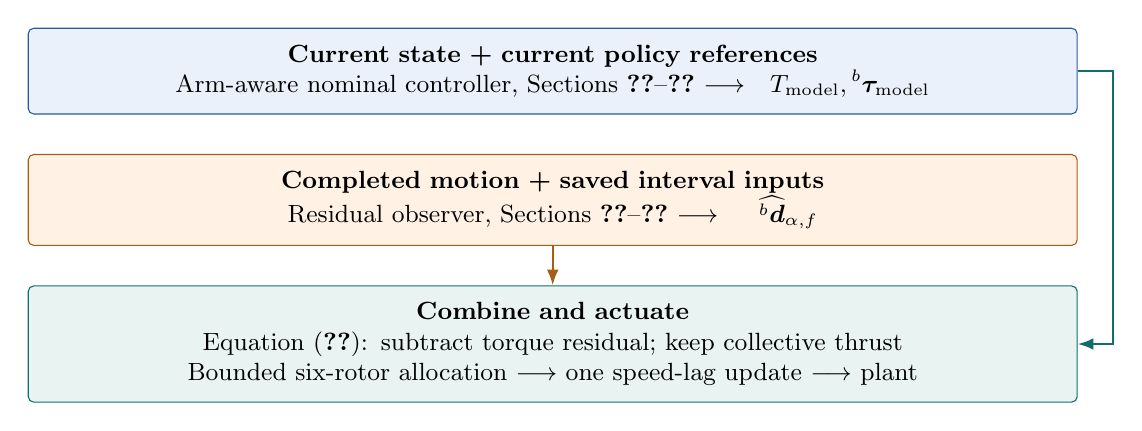
\begin{tikzpicture}
\node[model,text width=12.9cm] (nom) {\textbf{Current state + current policy references}\\
Arm-aware nominal controller, Sections~\ref{sec:model}--\ref{sec:nominal}
$\longrightarrow T_{\rm model},\bv\tau_{\rm model}$};
\node[obs,text width=12.9cm,below=5mm of nom] (obs) {\textbf{Completed motion + saved interval inputs}\\
Residual observer, Sections~\ref{sec:residual}--\ref{sec:discrete}
$\longrightarrow\widehat{\bv d}_{\alpha,f}$};
\node[box,text width=12.9cm,below=5mm of obs] (mix) {\textbf{Combine and actuate}\\
Equation~\eqref{eq:main}: subtract torque residual; keep collective thrust\\
Bounded six-rotor allocation $\longrightarrow$ one speed-lag update $\longrightarrow$ plant};
\draw[arr] (nom.east) -- ++(.45,0) |- (mix.east);
\draw[feedback] (obs)--(mix);
\end{tikzpicture}
\caption{Two paths into one rotor command. The predictive branch is immediate;
the feedback branch uses a completed interval and therefore has delay.}
\label{fig:overview}
\end{figure}

\clearpage
\textbf{Relation to the earlier report.} This is a self-contained companion to the earlier file, not an edit of it:
\begin{quote}\small\path{2026-11-04-borinot-model-wrench-illustrated.tex}\end{quote}
Its equation numbers start at (1) and are local to this document. The earlier
report derives the rigid-body model link by link. Here we rebuild the parts
needed to understand and implement the hybrid controller, then explain the
residual, timing, sensors and limits in detail.

\begingroup\small\setcounter{tocdepth}{1}\tableofcontents\endgroup
\clearpage

\section{Frames, controlled point and signals}\label{sec:frames}

The world frame $w$ is inertial. The base frame $b$ uses the rigid base axes.
All torques are about $C$, the \emph{base-only} centre of mass (CoM), not the
whole robot CoM and not necessarily the USD base-link origin.
\begin{equation}
\wv x=\Rw\,\bv x,\qquad
\bv x=\Rw^\top\wv x,\qquad
{}^b\mat R_w=\Rw^\top.
\label{eq:frames}
\end{equation}
The inner frame labels match. The matrix $\Rw$ maps base coordinates to world
coordinates. Its transpose maps in the opposite direction.

The motion variables are
\begin{equation}
\bv a=\Rw^\top\frac{d\wv v_C}{dt},\quad
\wv\Omega=\Rw\,\bv\Omega,\quad
\bv\alpha=\Rw^\top\frac{d\wv\Omega}{dt},\quad
\vct q=\begin{bmatrix}q_1&q_2\end{bmatrix}^{\!\top}.
\label{eq:accelerations}
\end{equation}
Here $\wv v_C$ is physical base-CoM velocity, $\bv\Omega$ is base angular
velocity and $\vct q$ contains the two joint angles. Linear acceleration is in
m/s$^2$; angular acceleration is in rad/s$^2$; angles are in rad.

Physical acceleration expressed in body axes is \emph{not} just the derivative
of body-frame velocity:
\begin{equation}
\bv a=\frac{d\bv v_C}{dt}+\bv\Omega\times\bv v_C,
\qquad \bv\alpha=\frac{d\bv\Omega}{dt}.
\label{eq:transport}
\end{equation}
The angular identity follows because $\bv\Omega\times\bv\Omega=0$.
We avoid a finite-difference version of the first transport term by differencing
world velocity directly. We also rotate gyro samples to world axes before their
finite difference.

To show the true dependencies, define the state tuple
\begin{equation}
\vct s=(\Rw,\bv\Omega,\vct q,\dot{\vct q}),\qquad
\bv g=\Rw^\top\wv g,\qquad \wv g=(0,0,-9.81)^\top\ {\rm m/s^2}.
\label{eq:state}
\end{equation}
The nominal mass matrix depends on configuration $\vct q$ only. Motion and
gravity enter its bias. Joint effort enters the reduced bias after joint
acceleration is eliminated. We suppress fixed calibration parameters as
function arguments, but not the changing state arguments.

\subsection{Signals we actually use}

\begin{longtable}{L{3.4cm}L{5.3cm}L{6.1cm}}
\toprule Signal & Predictive branch & Residual branch\\\midrule\endhead
Base attitude $\Rw$ & Rotate gravity/references; form attitude error & Put gyro in world axes; transform residuals\\
Body gyro $\bv\Omega$ & Motion bias and rate feedback & Two samples give an angular-acceleration estimate\\
Joint encoders $\vct q,\dot{\vct q}$ & Evaluate model and software PD & Saved model already includes their interval-start values\\
Base-CoM $\wv v_C$ & Not needed by the nominal law & Two samples give physical linear acceleration\\
Realized rotor speeds $\vct\omega_r$ & Motor state and policy observation & Reconstruct the torque that acted in the interval\\
Policy references & Current nominal request & Never used as measured acceleration\\
Hip load cell / simulator acceleration & Not used & Not used\\\bottomrule
\end{longtable}
A simulator velocity is an ideal state signal here. Hardware needs a measured or
estimated equivalent, with timestamp and sensor-position alignment.

\section{Recover the arm-aware reduced model}\label{sec:model}

\subsection{Start from the eight coupled equations}

Use physical base acceleration in base axes, followed by base angular
acceleration and two joint accelerations. The contact-free nominal model is
\begin{equation}
\underbrace{\begin{bmatrix}
\mat M_{bb}(\vct q)&\mat M_{bj}(\vct q)\\
\mat M_{jb}(\vct q)&\mat M_{jj}(\vct q)
\end{bmatrix}}_{\mat M(\vct q)\in\RR^{8\times8}}
\begin{bmatrix}\vct z_b\\\ddot{\vct q}\end{bmatrix}
+\begin{bmatrix}\vct h_b(\vct s)\\\vct h_j(\vct s)\end{bmatrix}
=\begin{bmatrix}\bv F_{\rm rot}\\\bv\tau_{\rm rot}\\\vct\tau_j\end{bmatrix},
\quad
\vct z_b=\begin{bmatrix}\bv a\\\bv\alpha\end{bmatrix}.
\label{eq:fullmodel}
\end{equation}
Subscript $b$ in these block indices means the six base coordinates;
$j$ means the two joint coordinates. The upper force rows have units N, the
upper moment rows have units N\,m, and the joint rows have units N\,m.
The symmetric off-diagonal blocks obey
$\mat M_{jb}(\vct q)=\mat M_{bj}(\vct q)^\top$.

The full matrix comes from summing each link's translated and rotated inertia.
It retains the free joints, the base--arm coupling and the declared joint
armature. The bias contains gravity, centripetal, Coriolis and gyroscopic terms.
It does not treat the arm as locked. These are the same nominal quantities used
by the existing model-wrench modes.

\subsection{Compute the bounded arm effort first}
\begin{equation}
\vct\tau_{j,\rm raw}
=k_p(\vct q_d-\vct q)-k_d\dot{\vct q},\qquad
\vct\tau_j=\operatorname{clip}
(\vct\tau_{j,\rm raw},-\tau_{j,\max},\tau_{j,\max}).
\label{eq:pd}
\end{equation}
Clipping is componentwise. We send this software PD effort to the joints at the
physics rate. Implicit joint stiffness and damping are zero, so a second PD
controller is not added by the simulator. The model uses the \emph{bounded}
effort, not the target angle alone and not an unbounded PD request.

\subsection{Eliminate joint acceleration without pretending it is independent}
The lower row of \eqref{eq:fullmodel} gives
\begin{equation}
\ddot{\vct q}=\mat M_{jj}(\vct q)^{-1}
\left[\vct\tau_j-\vct h_j(\vct s)-\mat M_{jb}(\vct q)\vct z_b\right].
\label{eq:ddq}
\end{equation}
This is not a separately known joint acceleration. It still depends on the
unknown base acceleration $\vct z_b$. We substitute it into the upper row.
The inverse is that of the $2\times2$ joint block, not a rectangular coupling block.
In code we use linear solves rather than explicitly forming this inverse.

\begin{equation}
\begin{aligned}
\mat E(\vct q)&=\mat M_{bb}(\vct q)
-\mat M_{bj}(\vct q)\mat M_{jj}(\vct q)^{-1}\mat M_{jb}(\vct q),\\
\vct\eta(\vct s,\vct\tau_j)&=\vct h_b(\vct s)
+\mat M_{bj}(\vct q)\mat M_{jj}(\vct q)^{-1}
\left[\vct\tau_j-\vct h_j(\vct s)\right].
\end{aligned}\label{eq:reduceddefinitions}
\end{equation}
The matrix $\mat E(\vct q)$ is a Schur complement: it is the effective base
inertia when the joints may accelerate. Only the bias also depends on joint
rates, body rate, gravity and the bounded applied effort.

Partition the reduced system into force and torque rows:
\begin{equation}
\begin{bmatrix}\bv F_{\rm rot}\\\bv\tau_{\rm rot}\end{bmatrix}
=\underbrace{\begin{bmatrix}
\mat E_{aa}(\vct q)&\mat E_{a\alpha}(\vct q)\\
\mat E_{\alpha a}(\vct q)&\mat E_{\alpha\alpha}(\vct q)
\end{bmatrix}}_{\mat E(\vct q)}
\begin{bmatrix}\bv a\\\bv\alpha\end{bmatrix}
+\begin{bmatrix}\vct\eta_a(\vct s,\vct\tau_j)\\
\vct\eta_\alpha(\vct s,\vct\tau_j)\end{bmatrix}.
\label{eq:reduced}
\end{equation}
Each block has size $3\times3$.
$\mat E_{aa}$ has units kg; $\mat E_{a\alpha}$ and $\mat E_{\alpha a}$ have
units kg\,m; $\mat E_{\alpha\alpha}$ has units kg\,m$^2$.
The arm affects \emph{every} block and the bias. It is not just an extra torque
that can be appended once at the end.

\begin{figure}[H]
\centering
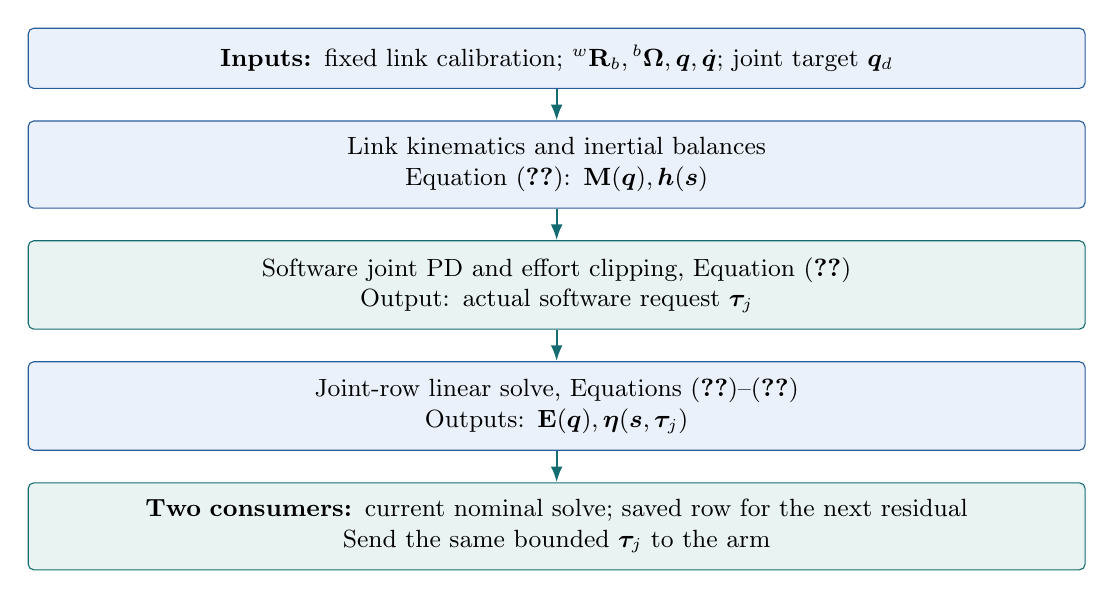
\begin{tikzpicture}[node distance=4mm]
\node[model,text width=13cm] (in) {\textbf{Inputs:} fixed link calibration;
$\Rw,\bv\Omega,\vct q,\dot{\vct q}$; joint target $\vct q_d$};
\node[model,text width=13cm,below=of in] (dyn) {Link kinematics and inertial balances\\
Equation~\eqref{eq:fullmodel}: $\mat M(\vct q),\vct h(\vct s)$};
\node[box,text width=13cm,below=of dyn] (pd) {Software joint PD and effort clipping,
Equation~\eqref{eq:pd}\\Output: actual software request $\vct\tau_j$};
\node[model,text width=13cm,below=of pd] (reduce) {Joint-row linear solve,
Equations~\eqref{eq:ddq}--\eqref{eq:reduceddefinitions}\\
Outputs: $\mat E(\vct q),\vct\eta(\vct s,\vct\tau_j)$};
\node[box,text width=13cm,below=of reduce] (out) {\textbf{Two consumers:}
current nominal solve; saved row for the next residual\\
Send the same bounded $\vct\tau_j$ to the arm};
\draw[arr] (in)--(dyn);\draw[arr] (dyn)--(pd);\draw[arr] (pd)--(reduce);\draw[arr] (reduce)--(out);
\end{tikzpicture}
\caption{Inputs and outputs of the dynamics reduction. The effort used in the
model is also the effort sent to the arm. Saved quantities must travel together.}
\label{fig:model}
\end{figure}

\section{The nominal controller is retained}\label{sec:nominal}

\subsection{Policy interfaces}
\begin{equation}
\begin{aligned}
\text{Heading variant}:\quad&
[\wv a_d\ (3),\ \psi_d\ (1),\ \bv\Omega_d\ (3),\ \vct q_d\ (2)],\\
\text{Yawless variant}:\quad&
[\wv a_d\ (3),\ \bv\Omega_d\ (3),\ \vct q_d\ (2)].
\end{aligned}\label{eq:actions}
\end{equation}
There are nine or eight scalar outputs. $\psi_d$ is a world heading angle.
PPO sends physical references: m/s$^2$, rad, rad/s and rad.
SAC sends normalized scalar references, using the same existing scales in
\texttt{env.wrench} and \texttt{env.body\_rate\_scale}.
The headed SAC heading is an offset from the configured home yaw; the headed
PPO heading is the absolute world angle. Neither convention is changed here.

Optional $(\cos,\sin)$ pairs replace supported scalar angles in place. They
decode to radians and bypass that angle's scalar scale. A zero pair means zero
radians. The yawless mode has no heading output, so it rejects the yaw-pair flag.
Joint pairs remain available in both modes. Arm hold replaces both joint targets
with zero before the PD law.

\subsection{Choose a virtual force direction, not an impossible actuator force}
Transform the policy acceleration into current body axes:
\begin{equation}
\bv a_d=\Rw^\top\wv a_d,\qquad
\wv F_v=\Rw\left[
\mat E_{aa}(\vct q)\bv a_d+
\mat E_{a\alpha}(\vct q)\bv\alpha_v+
\vct\eta_a(\vct s,\vct\tau_j)\right].
\label{eq:virtualforce}
\end{equation}
By default $\bv\alpha_v=0$. This is a \emph{direction-building choice}; it does
not impose zero actual angular acceleration. The optional
\texttt{model\_wrench\_use\_prev\_alpha=True} substitutes the previous physics
tick's desired body-axis angular-acceleration components. This is a delayed
reference heuristic, not a same-tick coupled solve or a measured acceleration.
The existing option is retained in both hybrids.

Let $\e=(0,0,1)^\top$ denote the canonical third-axis coordinate vector. The
desired world thrust direction is
\begin{equation}
\wv z_d=\frac{\wv F_v}{\|\wv F_v\|}.
\label{eq:direction}
\end{equation}
At near-zero force, retain the current thrust axis. The desired direction is
not yet the force that the robot can produce at its current attitude.

\subsection{Heading mode: construct an attitude, then angular acceleration}
For nondegenerate directions, the heading completion is
\begin{equation}
\begin{gathered}
\wv h_x=(\cos\psi_d,\sin\psi_d,0)^\top,\quad
\wv y_d=\frac{\wv z_d\times\wv h_x}{\|\wv z_d\times\wv h_x\|},\quad
\wv x_d=\wv y_d\times\wv z_d,\\
{}^w\mat R_{b^*}=[\wv x_d\ \wv y_d\ \wv z_d],\qquad
\Delta\mat R={}^b\mat R_{b^*}=\Rw^\top{}^w\mat R_{b^*}.
\end{gathered}\label{eq:heading}
\end{equation}
If the cross product is too small, the implementation uses the perpendicular
horizontal heading vector instead. The frame $b^*$ is the desired base frame.

The default geometric attitude error splits the unit error quaternion
$\vct Q_e=(w_e,x_e,y_e,z_e)$ of $\Delta\mat R$ into swing and twist:
\begin{equation}
\begin{gathered}
\vct Q_z=\frac{(w_e,0,0,z_e)}{\sqrt{w_e^2+z_e^2}},\qquad
\vct Q_t=\vct Q_e\otimes\vct Q_z^{-1},\\
\bv\alpha_d=k_t\operatorname{Log}(\vct Q_t)
+k_\psi\operatorname{Log}(\vct Q_z)
+\mat K_\Omega(\bv\Omega_d-\bv\Omega).
\end{gathered}\label{eq:headedalpha}
\end{equation}
$\otimes$ is quaternion multiplication. $\operatorname{Log}$ returns the full-angle
principal rotation vector in current body axes, not a half-angle vector. At the
undefined inverted-axis twist, the implementation chooses identity twist.
The existing \texttt{method\_1} and \texttt{method\_2} alternatives remain available;
the hybrid does not alter them.

\subsection{Yawless mode: only align the thrust axis}
Define the target thrust direction written in the current body axes, then find
the shortest rotation that sends the current third axis to it:
\begin{equation}
\begin{gathered}
\bv z_d=\Rw^\top\wv z_d,\quad
\bv v_t=\e\times\bv z_d,\quad
\theta=\operatorname{atan2}(\|\bv v_t\|,\e^\top\bv z_d),\\
\bv e_t=\frac{\theta}{\|\bv v_t\|}\bv v_t,\qquad
\bv\alpha_d=k_t\bv e_t+\mat K_\Omega(\bv\Omega_d-\bv\Omega).
\end{gathered}\label{eq:yawlessalpha}
\end{equation}
At aligned axes the error is zero. At an exact antipode a body-$x$ half-turn
breaks the tie. The third component of $\bv e_t$ is zero, but the third component
of $\bv\alpha_d$ generally is not. We retain body-$z$ rate control, gyroscopic
terms and arm coupling. Yawless means no heading-angle restoring target; it does
not mean fixed Euler yaw or zero yaw torque.

\subsection{Solve the instantaneous actuator-compatible wrench}
All six propellers push along the \emph{current} body $z$-axis:
\begin{equation}
\bv F_{\rm rot}=T\e,\qquad
T\e=\mat E_{aa}(\vct q)\bv a_*
+\mat E_{a\alpha}(\vct q)\bv\alpha_d
+\vct\eta_a(\vct s,\vct\tau_j).
\label{eq:thrustaxis}
\end{equation}
There are four unknowns: the three components of $\bv a_*$ and scalar $T$.
There are only three force equations. We close the system with
\begin{equation}
\e^\top\bv a_*=\e^\top\bv a_d.
\label{eq:closure}
\end{equation}
This is acceleration along the \emph{current body axis}, not world vertical.
The subscript $*$ means the nominal pre-limit acceleration chosen by this solve.

Set
\begin{equation}
\begin{aligned}
\bv c(\vct s,\vct\tau_j,\bv\alpha_d)&=
\mat E_{a\alpha}(\vct q)\bv\alpha_d+\vct\eta_a(\vct s,\vct\tau_j),\\
\bv p(\vct q)&=\mat E_{aa}(\vct q)^{-1}\e,\qquad
\bv r(\vct s,\vct\tau_j,\bv\alpha_d)=
\mat E_{aa}(\vct q)^{-1}\bv c(\vct s,\vct\tau_j,\bv\alpha_d),\\
T_{\rm model}&=\frac{\e^\top\bv a_d+
\e^\top\bv r(\vct s,\vct\tau_j,\bv\alpha_d)}{\e^\top\bv p(\vct q)},\\
\bv a_*&=\bv p(\vct q)T_{\rm model}-
\bv r(\vct s,\vct\tau_j,\bv\alpha_d).
\end{aligned}\label{eq:forcesolve}
\end{equation}
The nominal torque then follows from the reduced rotational row:
\begin{equation}
\boxed{\bv\tau_{\rm model}=
\mat E_{\alpha a}(\vct q)\bv a_*
+\mat E_{\alpha\alpha}(\vct q)\bv\alpha_d
+\vct\eta_\alpha(\vct s,\vct\tau_j).}
\label{eq:nominaltorque}
\end{equation}
This is the same request the original model-wrench controller computes.
Equation~\eqref{eq:main} changes only what we send to the allocator afterward.
Predicted base and joint accelerations in controller diagnostics remain nominal.
They are not predictions after correction, saturation and motor lag.

\begin{figure}[H]
\centering
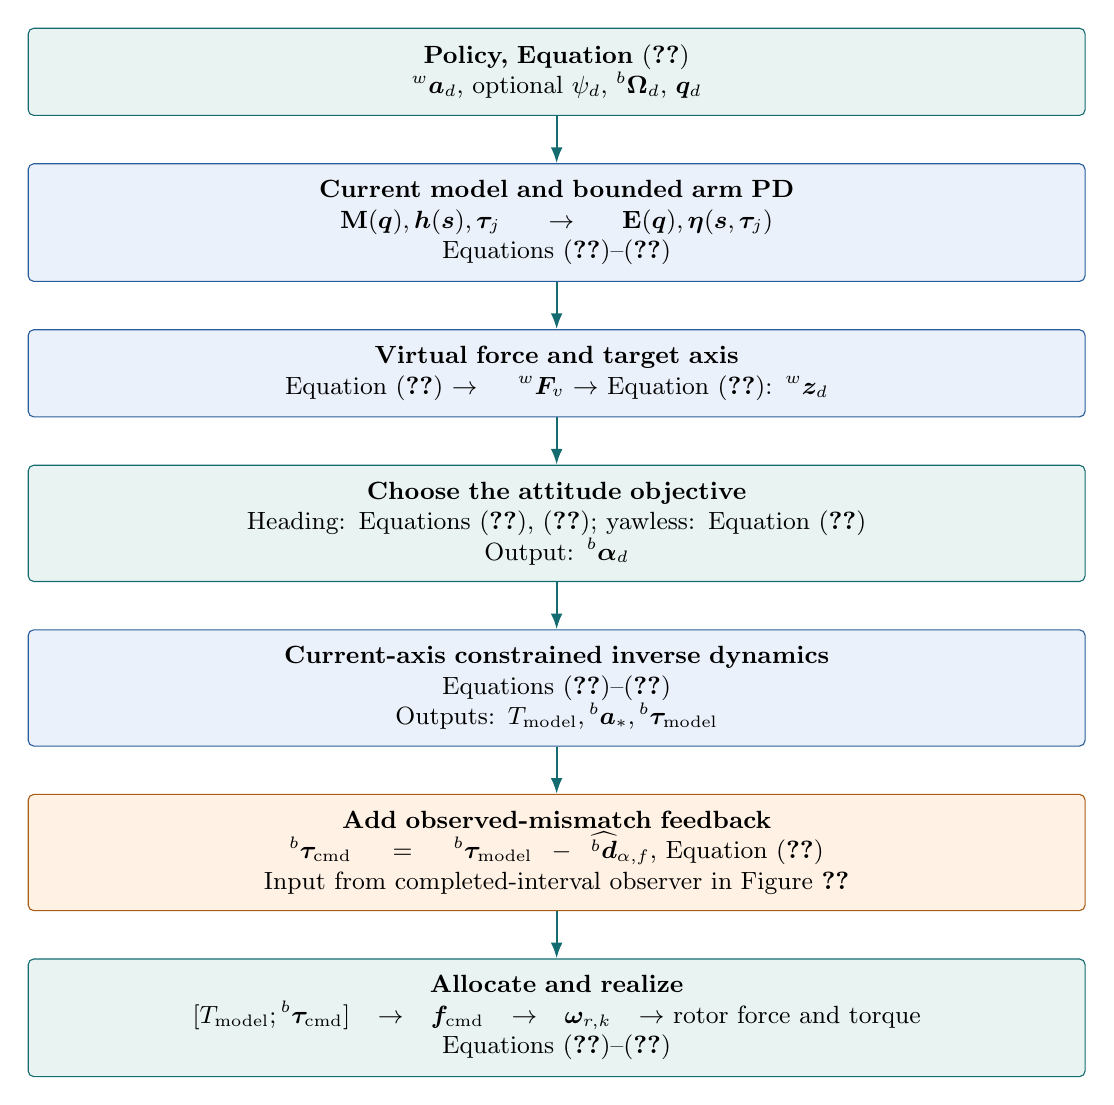
\begin{tikzpicture}[node distance=6mm]
\node[box,text width=13cm] (policy) {\textbf{Policy, Equation~\eqref{eq:actions}}\\
$\wv a_d$, optional $\psi_d$, $\bv\Omega_d$, $\vct q_d$};
\node[model,text width=13cm,below=of policy] (model) {\textbf{Current model and bounded arm PD}\\
$\mat M(\vct q),\vct h(\vct s),\vct\tau_j\to
\mat E(\vct q),\vct\eta(\vct s,\vct\tau_j)$\\
Equations~\eqref{eq:fullmodel}--\eqref{eq:reduced}};
\node[model,text width=13cm,below=of model] (dir) {\textbf{Virtual force and target axis}\\
Equation~\eqref{eq:virtualforce} $\to\wv F_v$
$\to$ Equation~\eqref{eq:direction}: $\wv z_d$};
\node[box,text width=13cm,below=of dir] (att) {\textbf{Choose the attitude objective}\\
Heading: Equations~\eqref{eq:heading}, \eqref{eq:headedalpha};
yawless: Equation~\eqref{eq:yawlessalpha}\\
Output: $\bv\alpha_d$};
\node[model,text width=13cm,below=of att] (solve) {\textbf{Current-axis constrained inverse dynamics}\\
Equations~\eqref{eq:thrustaxis}--\eqref{eq:nominaltorque}\\
Outputs: $T_{\rm model},\bv a_*,\bv\tau_{\rm model}$};
\node[obs,text width=13cm,below=of solve] (cor) {\textbf{Add observed-mismatch feedback}\\
$\bv\tau_{\rm cmd}=\bv\tau_{\rm model}-\widehat{\bv d}_{\alpha,f}$,
Equation~\eqref{eq:main}\\Input from completed-interval observer in Figure~\ref{fig:observer}};
\node[box,text width=13cm,below=of cor] (rot) {\textbf{Allocate and realize}\\
$[T_{\rm model};\bv\tau_{\rm cmd}]\to\vct f_{\rm cmd}\to\vct\omega_{r,k}
\to$ rotor force and torque\\Equations~\eqref{eq:allocate}--\eqref{eq:realized}};
\draw[arr] (policy)--(model);\draw[arr] (model)--(dir);\draw[arr] (dir)--(att);
\draw[arr] (att)--(solve);\draw[arr] (solve)--(cor);\draw[arr] (cor)--(rot);
\end{tikzpicture}
\caption{Detailed current-tick input/output chain. State and fixed calibration
enter the blue model blocks. The orange block is the only new torque change.
The joint-effort path goes directly from the PD block to the plant as well.}
\label{fig:nominal}
\end{figure}

\section{What torque is reconstructed from the rotors?}\label{sec:rotors}

Let $\vct f=(f_1,\ldots,f_6)^\top$ be the six positive rotor thrusts, in N.
Let $\bv r_i$ be rotor $i$'s position relative to the nominal base CoM. Define
\begin{equation}
\mat A=\begin{bmatrix}
1&\cdots&1\\
r_{1,y}&\cdots&r_{6,y}\\
-r_{1,x}&\cdots&-r_{6,x}\\
\sigma_1 k_m/k_f&\cdots&\sigma_6 k_m/k_f
\end{bmatrix},\qquad
\begin{bmatrix}T\\\bv\tau_{\rm rot}\end{bmatrix}=\mat A\vct f.
\label{eq:mixer}
\end{equation}
$\sigma_i\in\{-1,+1\}$ is the configured aerodynamic torque sign. Lever arms
supply roll and pitch torque. The last row supplies the aerodynamic drag torque.
The last three rows are denoted $\mat A_\tau$.

The general rotor-spin bookkeeping discussed in chat can be written
\begin{equation}
\bv\tau_{\rm rot}=\mat G_1(\vct\omega_r\odot\vct\omega_r)
+\mat G_2\dot{\vct\omega}_r,\qquad
\mat G_1=k_f\mat A_\tau.
\label{eq:generalrotor}
\end{equation}
$\odot$ means elementwise multiplication. Rotor-speed magnitudes
$\omega_{r,i}$ have units rad/s, and $f_i=k_f\omega_{r,i}^2$.
$\mat G_2$ would map rotor angular acceleration to reaction torque on the base.
Its signed columns depend on rotor angular momentum conventions. This is
\emph{rotor} dynamics, not arm dynamics.

\textbf{Actual implementation:} the model-wrench plant and allocator have no
identified rotor-spin term, so $\mat G_2=0$. We preserve that choice. The new
hybrids use \eqref{eq:mixer} with post-lag speeds. A nonzero setting under
\texttt{env.indi} belongs to the separate standalone INDI controller and does not
activate a spin model here. A calibrated extension must change the reconstructed
torque, actual plant torque and dynamic allocation consistently.

The rotor torque is usually an \emph{estimate} based on speed and a calibrated
map. No torque transducer measures it. If geometry, aerodynamic coefficients,
rotor speeds or base CoM are wrong, the reconstructed value is wrong too.
The residual can then include those errors. We never add a modelled arm reaction
to \eqref{eq:mixer} or \eqref{eq:generalrotor}.

\section{Derive the disturbance correction}\label{sec:residual}

\subsection{Observed dynamics versus desired dynamics}
Collect unknown effects into an equivalent reduced torque $\bv d_\alpha$:
\begin{equation}
\bv\tau_{\rm rot}+\bv d_\alpha=
\mat E_{\alpha a}(\vct q)\bv a_{\rm obs}
+\mat E_{\alpha\alpha}(\vct q)\bv\alpha_{\rm obs}
+\vct\eta_\alpha(\vct s,\vct\tau_j).
\label{eq:observedbalance}
\end{equation}
The subscript ``obs'' means observed motion, never a policy reference or the
inverse model's solved acceleration. Our sign convention puts a helping external
torque on the left. A positive helping torque should reduce the rotor request.
Rearranging gives the instantaneous residual
\begin{equation}
\bv r_d=
\mat E_{\alpha a}(\vct q)\bv a_{\rm obs}
+\mat E_{\alpha\alpha}(\vct q)\bv\alpha_{\rm obs}
+\vct\eta_\alpha(\vct s,\vct\tau_j)-\bv\tau_{\rm rot}.
\label{eq:rawcontinuous}
\end{equation}
It has units N\,m. Both measured linear acceleration and angular acceleration
matter because this is the \emph{reduced coupled} rotational row.

For constant axes and synchronized samples, a convenient notation is
\begin{equation}
\widehat{\bv d}_{\alpha,f}=\mathcal H[\bv r_d],\qquad
\bv\tau_{\rm cmd}=\bv\tau_{\rm model}-\widehat{\bv d}_{\alpha,f}.
\label{eq:continuouscorrection}
\end{equation}
$\mathcal H$ denotes a common linear low-pass filter. For rotating body axes the
implementation instead filters the world residual and then rotates it back;
Section~\ref{sec:discrete} gives that exact discrete operation.

\subsection{Why this keeps the fast arm prediction}
With locally constant matrices, let a subscript $f$ mean a common filter on a
signal and freeze $\mat E$ over that filter memory. Expanding
\eqref{eq:continuouscorrection} gives
\begin{equation}
\begin{aligned}
\bv\tau_{\rm cmd}={}&\bv\tau_{{\rm rot},f}
+\mat E_{\alpha\alpha}(\vct q)
(\bv\alpha_d-\bv\alpha_{{\rm obs},f})\\
&+\mat E_{\alpha a}(\vct q)(\bv a_*-\bv a_{{\rm obs},f})
+\left[\vct\eta_\alpha(\vct s,\vct\tau_j)
-\vct\eta_{\alpha,f}\right].
\end{aligned}\label{eq:expanded}
\end{equation}
The first line resembles an INDI angular increment. The second keeps the
predictable changes in translation--rotation coupling and arm bias. We do not
wait for an unknown-disturbance estimator to rediscover a known arm command.

Equation~\eqref{eq:expanded} is an explanatory local approximation, not the code.
For changing configurations,
\begin{equation}
\mathcal H[\mat E_{\alpha a}(\vct q(t))\bv a(t)]
\ne\mat E_{\alpha a}(\vct q(t))\mathcal H[\bv a(t)]
\quad\hbox{in general}.
\label{eq:noncommute}
\end{equation}
The same warning applies to the rotational block and changing coordinate
rotations. The implementation forms the complete torque residual before
filtering it. It never pulls a changing dynamics matrix outside the filter.

\subsection{What an ``equivalent disturbance'' contains}
Suppose the full dynamics also have an unknown generalized base input
$\vct d_b\in\RR^6$ and joint input $\vct d_j\in\RR^2$ on their right-hand side.
Eliminating the joint row yields
\begin{equation}
\vct d_{\rm eff}=\vct d_b-
\mat M_{bj}(\vct q)\mat M_{jj}(\vct q)^{-1}\vct d_j.
\label{eq:effectiveexternal}
\end{equation}
The last three components contribute to $\bv d_\alpha$. Thus an arm contact or
joint-effort mismatch may appear through the reduction, not only as a direct
external base torque. Model and sensor errors also enter the estimated residual.
It is not an isolated force sensor or a perfect contact-torque measurement.

If the model and sensing are exact and the discrete motion agrees with the
saved dynamics, the residual is zero and the original model-wrench request is
recovered. On a real finite-step rollout, zero physical disturbance alone does
not guarantee exactly zero residual. Slowly changing unknown torque is the
most favorable case for this observer. A sharp impact violates that assumption.

\section{The exact causal discrete observer}\label{sec:discrete}

\subsection{Which instant does each quantity belong to?}
Let $t_k=k\Delta t$, where $\Delta t=1/f_{\rm physics}$. At the start of tick $k$
we have just observed the motion caused by commands held over
$[t_{k-1},t_k]$. Those commands were computed one tick earlier.
We save $\mat E(\vct q_{k-1})$ and
$\vct\eta(\vct s_{k-1},\vct\tau_{j,k-1})$, including the bounded effort actually
sent. We also save the realized rotor torque \emph{after} its motor-speed update.

\begin{figure}[H]
\centering
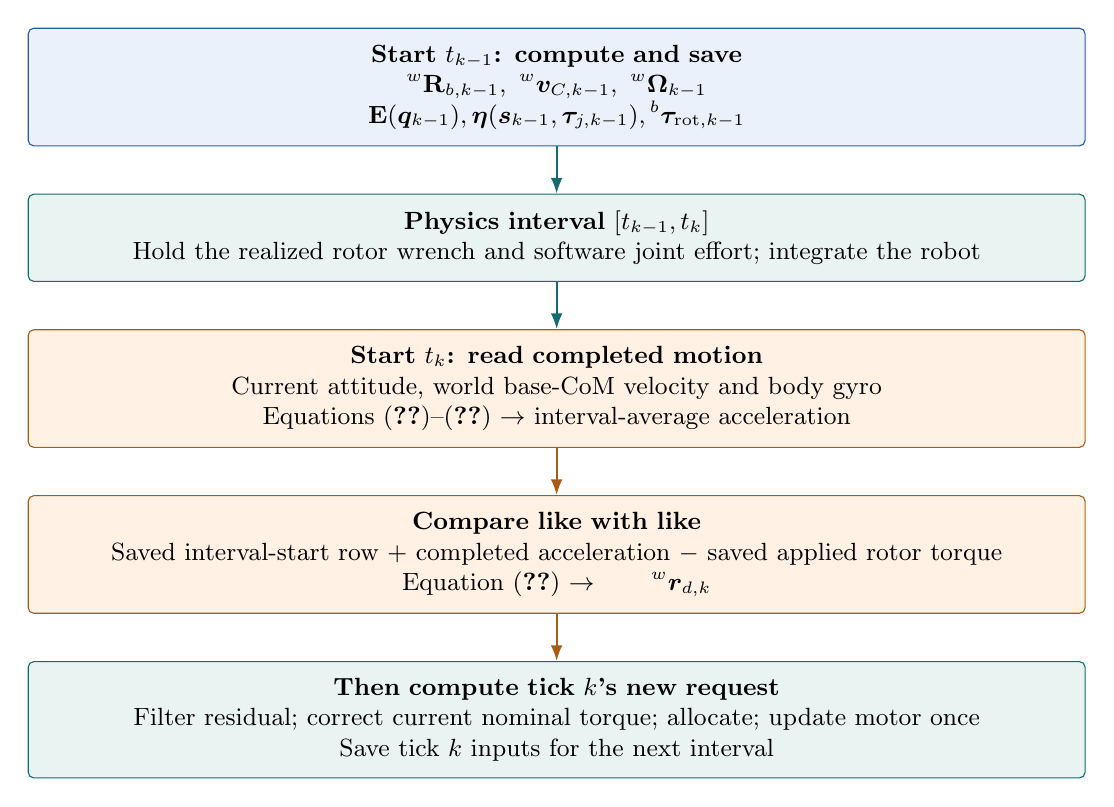
\begin{tikzpicture}[node distance=6mm]
\node[model,text width=13cm] (old) {\textbf{Start $t_{k-1}$: compute and save}\\
$\Rk{k-1},\ \wv v_{C,k-1},\ \wv\Omega_{k-1}$\\
$\mat E(\vct q_{k-1}),\vct\eta(\vct s_{k-1},\vct\tau_{j,k-1}),\bv\tau_{{\rm rot},k-1}$};
\node[box,text width=13cm,below=of old] (int) {\textbf{Physics interval $[t_{k-1},t_k]$}\\
Hold the realized rotor wrench and software joint effort; integrate the robot};
\node[obs,text width=13cm,below=of int] (new) {\textbf{Start $t_k$: read completed motion}\\
Current attitude, world base-CoM velocity and body gyro\\
Equations~\eqref{eq:increments}--\eqref{eq:bodyincrements} $\to$
interval-average acceleration};
\node[obs,text width=13cm,below=of new] (res) {\textbf{Compare like with like}\\
Saved interval-start row + completed acceleration $-$ saved applied rotor torque\\
Equation~\eqref{eq:discreteraw} $\to\wv r_{d,k}$};
\node[box,text width=13cm,below=of res] (cmd) {\textbf{Then compute tick $k$'s new request}\\
Filter residual; correct current nominal torque; allocate; update motor once\\
Save tick $k$ inputs for the next interval};
\draw[arr] (old)--(int);\draw[arr] (int)--(new);\draw[feedback] (new)--(res);\draw[feedback] (res)--(cmd);
\end{tikzpicture}
\caption{The one-interval timing contract. A new arm target at $t_k$ must not
replace $\vct\tau_{j,k-1}$ in the residual for the completed interval.}
\label{fig:timing}
\end{figure}

\subsection{Recover physical interval-average accelerations}
First rotate each gyro sample using its \emph{own} attitude. Then difference in
world axes:
\begin{equation}
\begin{aligned}
\wv\Omega_k&=\Rk{k}\,{}^b\vct\Omega_k,\\
\wv{\bar a}_k&=\frac{\wv v_{C,k}-\wv v_{C,k-1}}{\Delta t},\\
\wv{\bar\alpha}_k&=\frac{\wv\Omega_k-\wv\Omega_{k-1}}{\Delta t}.
\end{aligned}\label{eq:increments}
\end{equation}
The bars indicate averages over the completed interval. No model prediction or
policy output supplies either numerator. Now express both averages in the
\emph{saved interval-start} body axes:
\begin{equation}
{}^{b_{k-1}}\vct{\bar a}_k=\Rk{k-1}^\top\wv{\bar a}_k,
\qquad
{}^{b_{k-1}}\vct{\bar\alpha}_k=\Rk{k-1}^\top\wv{\bar\alpha}_k.
\label{eq:bodyincrements}
\end{equation}
This notation distinguishes the time-dependent axes explicitly. Current gyro
components must not be directly subtracted from old components while claiming
they are vectors in one fixed frame.

\subsection{Apply the saved complete torque row}
\begin{equation}
\begin{aligned}
{}^{b_{k-1}}\vct r_{d,k}={}&
\mat E_{\alpha a}(\vct q_{k-1})\,{}^{b_{k-1}}\vct{\bar a}_k\\
&+\mat E_{\alpha\alpha}(\vct q_{k-1})\,{}^{b_{k-1}}\vct{\bar\alpha}_k\\
&+\vct\eta_\alpha(\vct s_{k-1},\vct\tau_{j,k-1})
-{}^{b_{k-1}}\vct\tau_{{\rm rot},k-1},\\
\wv r_{d,k}={}&\Rk{k-1}\,{}^{b_{k-1}}\vct r_{d,k}.
\end{aligned}\label{eq:discreteraw}
\end{equation}
The code saves just the last three rows of $\mat E$, the torque bias and the
needed histories. There is no second model evaluation for the old interval.
The world-frame residual in the last line is the input to the filter.

\subsection{Filter in fixed axes; correct in current axes}
\begin{equation}
\begin{aligned}
\widehat{\wv d}_{\alpha,f,k}&=\mathcal H_d[\wv r_d]_k,\\
\widehat{{}^{b_k}\vct d}_{\alpha,f,k}&=\Rk{k}^\top\widehat{\wv d}_{\alpha,f,k},\\
{}^{b_k}\vct\tau_{{\rm cmd},k}&={}^{b_k}\vct\tau_{{\rm model},k}
-\widehat{{}^{b_k}\vct d}_{\alpha,f,k}.
\end{aligned}
\label{eq:discretecorrection}
\end{equation}
$\mathcal H_d$ is one identical scalar filter per world component. Filtering the
complete residual with the same linear filter is equivalent to filtering its
complete model-torque and rotor-torque signals with matching histories and then
subtracting them. It is not equivalent to separately filtering velocities,
squaring filtered rotor speeds, or evaluating matrices at the latest state.

A world-fixed disturbance stays fixed in the filter even while the robot turns.
A body-fixed disturbance rotates in world axes and therefore still experiences
filter delay. There is no globally frame-independent low-pass filter for every
possible changing disturbance direction; the chosen fixed axes make the
operation unambiguous.

\begin{figure}[H]
\centering
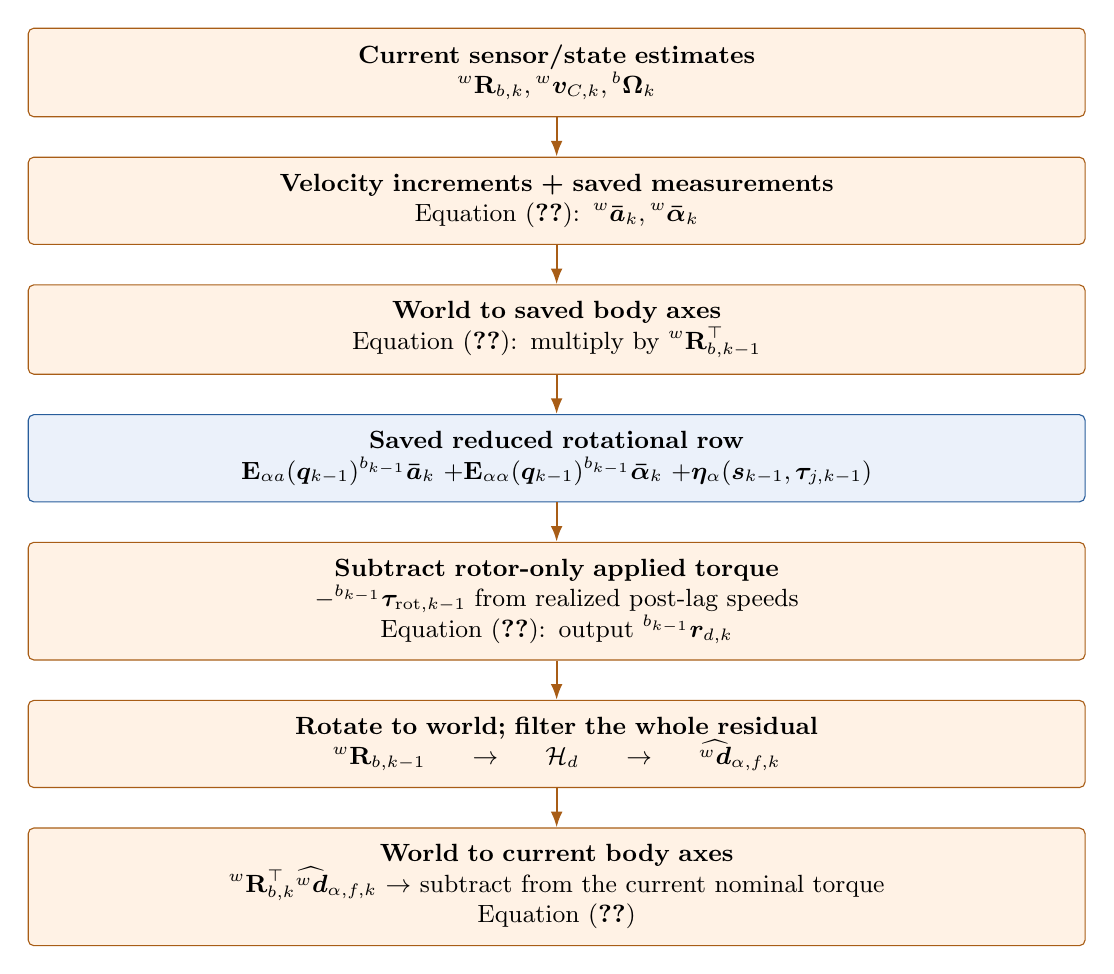
\begin{tikzpicture}[node distance=5mm]
\node[obs,text width=13cm] (sensors) {\textbf{Current sensor/state estimates}\\
$\Rk{k},\wv v_{C,k},{}^b\vct\Omega_k$};
\node[obs,text width=13cm,below=of sensors] (diff) {\textbf{Velocity increments + saved measurements}\\
Equation~\eqref{eq:increments}: $\wv{\bar a}_k,\wv{\bar\alpha}_k$};
\node[obs,text width=13cm,below=of diff] (oldframe) {\textbf{World to saved body axes}\\
Equation~\eqref{eq:bodyincrements}: multiply by $\Rk{k-1}^\top$};
\node[model,text width=13cm,below=of oldframe] (row) {\textbf{Saved reduced rotational row}\\
$\mat E_{\alpha a}(\vct q_{k-1}){}^{b_{k-1}}\vct{\bar a}_k$
$+\mat E_{\alpha\alpha}(\vct q_{k-1}){}^{b_{k-1}}\vct{\bar\alpha}_k$
$+\vct\eta_\alpha(\vct s_{k-1},\vct\tau_{j,k-1})$};
\node[obs,text width=13cm,below=of row] (sub) {\textbf{Subtract rotor-only applied torque}\\
$-{}^{b_{k-1}}\vct\tau_{{\rm rot},k-1}$ from realized post-lag speeds\\
Equation~\eqref{eq:discreteraw}: output ${}^{b_{k-1}}\vct r_{d,k}$};
\node[obs,text width=13cm,below=of sub] (filter) {\textbf{Rotate to world; filter the whole residual}\\
$\Rk{k-1}\to\mathcal H_d\to\widehat{\wv d}_{\alpha,f,k}$};
\node[obs,text width=13cm,below=of filter] (back) {\textbf{World to current body axes}\\
$\Rk{k}^\top\widehat{\wv d}_{\alpha,f,k}$
$\to$ subtract from the current nominal torque\\Equation~\eqref{eq:discretecorrection}};
\draw[feedback] (sensors)--(diff);\draw[feedback] (diff)--(oldframe);
\draw[feedback] (oldframe)--(row);\draw[feedback] (row)--(sub);
\draw[feedback] (sub)--(filter);\draw[feedback] (filter)--(back);
\end{tikzpicture}
\caption{Detailed observer input/output chain. Blue is the saved model; orange
is motion feedback and time alignment. There is no arm torque added to the
rotor estimate and no new-reference input to the old interval's balance.}
\label{fig:observer}
\end{figure}

\subsection{The filter used by the code}
The filter is a second-order Butterworth low-pass filter, using the bilinear
transform. With cutoff $f_c$ and physics interval $\Delta t$, define
\begin{equation}
\begin{gathered}
\kappa=\tan(\pi f_c\Delta t),\qquad
N=1+\sqrt2\kappa+\kappa^2,\\
b_0=\kappa^2/N,\quad b_1=2b_0,\quad b_2=b_0,\\
a_1=2(\kappa^2-1)/N,\qquad
a_2=(1-\sqrt2\kappa+\kappa^2)/N.
\end{gathered}\label{eq:coefficients}
\end{equation}
For each component of the raw world torque $x_k$ and filtered torque $y_k$,
\begin{equation}
y_k=b_0x_k+b_1x_{k-1}+b_2x_{k-2}-a_1y_{k-1}-a_2y_{k-2}.
\label{eq:filter}
\end{equation}
The implementation uses the equivalent transposed direct-form-II recurrence,
with two memory vectors. The cutoff is
\texttt{env.model\_wrench\_indi.filter\_cutoff\_hz}, default $12$ Hz.
Validation requires $0<f_c<f_{\rm physics}/2$.
At the default $200$ Hz physics rate, the timestep is $0.005$ s.

A larger cutoff responds sooner but passes more differentiated measurement
noise. A smaller cutoff reduces noise but adds delay. This parameter has no
universal best value. We do not change the existing attitude/rate gains to
compensate for it automatically.

\subsection{Approximation and numerical sensitivity}
Equation~\eqref{eq:increments} is an exact velocity-increment identity for an
interval mean in world axes. Equation~\eqref{eq:discreteraw} then applies a
\emph{frozen interval-start} model to that mean. For smoothly changing dynamics
this is a finite-step approximation; it is not the integral of the complete
changing model product over the interval.

The approximation includes changes in joint geometry, rates and body axes
during that step, as well as the simulator's integration choices. An impulse or
joint stop can make it much worse. Very small velocity increments in float32
also suffer subtraction roundoff before division by $\Delta t$. More frequent
sampling is not a free cure for noisy velocity estimates.

The model assumes the software joint effort acts over the interval. Friction,
armature approximation, effort lag, hard stops or unmodelled joint contacts can
violate that assumption. They can enter the residual as effective torque error.

\subsection{Reset behavior}
A physical reset clears the observer's previous velocity, gyro, attitude,
reduced row, bias, applied wrench and filter state for selected environments
only. A validity flag prevents differentiation across a teleport.
On the first tick the raw residual and correction are zero, so the request is
exactly the corresponding nominal mode. The controller then saves a fresh
interval. The next physics tick may use its completed motion.

A GoTo target change without a physical robot reset does not clear this history.
The robot motion is continuous. Erasing a valid observer every time the goal
clock changes would create unnecessary blind intervals.

\section{Allocation, motor lag and the actual plant input}\label{sec:allocation}

We combine the untouched collective with the corrected torque into the four
channels $\vct u_{\rm req}=[T_{\rm model};\bv\tau_{\rm cmd}]$. The existing
allocator approximately solves the bounded least-squares problem
\begin{equation}
\begin{aligned}
\vct f_{\rm cmd}&\simeq\underset{0\le f_i\le f_{\max}}{\operatorname{argmin}}
\left\|\mat W^{1/2}\mat S^{-1}
(\mat A\vct f-\vct u_{\rm req})\right\|_2^2,\\
\mat W&=\operatorname{diag}(w_T,w_x,w_y,w_z),\qquad
S_{\ell\ell}=f_{\max}\sum_{i=1}^{6}|A_{\ell i}|.
\end{aligned}\label{eq:allocate}
\end{equation}
Indices $\ell=1,\ldots,4$ enumerate collective and three torques. The normalizing
matrix $\mat S$ contains channel capacities. The weights come from
\texttt{env.wrench.allocation\_weights}. A fixed number of accelerated projected
iterations keeps the operation batched. The defaults remain 128 iterations and
weights $(1,10,10,1)$. This is not an equality solver for infeasible requests.

The motor lag acts on rotor speed, not thrust:
\begin{equation}
\begin{gathered}
\gamma=\begin{cases}
1,&\tau_m=0,\\
1-\exp(-\Delta t/\tau_m),&\tau_m>0,
\end{cases}\qquad
\vct\omega_{{\rm cmd},k}=\sqrt{\vct f_{{\rm cmd},k}/k_f},\\
\vct\omega_{r,k}=\vct\omega_{r,k-1}+
\gamma(\vct\omega_{{\rm cmd},k}-\vct\omega_{r,k-1}).
\end{gathered}\label{eq:motor}
\end{equation}
The square root is componentwise and $\tau_m$ is the existing motor time
constant, in seconds. The controller advances this state once. The environment
uses it directly and does not apply another motor filter.

The rotor-only wrench reconstructed for the next observer interval is
\begin{equation}
\vct f_{{\rm act},k}=k_f(\vct\omega_{r,k}\odot\vct\omega_{r,k}),\quad
\vct u_{{\rm act},k}=\mat A\vct f_{{\rm act},k},\quad
\bv\tau_{{\rm rot},k}=(\vct u_{{\rm act},k})_{2:4}.
\label{eq:realized}
\end{equation}
The index $2{:}4$ here is mathematical one-based indexing: the last three wrench
entries. This saved wrench is not the newest requested wrench and not the
pre-lag bounded allocation.

If the plant has a different actual base CoM or rotor map, the saved nominal
estimate need not equal the true applied moment. That mismatch is deliberately
not removed by reading randomized plant parameters into the nominal controller.

\textbf{Saturation matters.} The allocator may trade collective error for torque
error under its weights. Thus keeping the requested collective unchanged does
not guarantee identical realized collective after a torque correction. The
rotation-only description refers to the requested wrench before allocation.
The diagnostic \texttt{allocation\_residual} is pre-lag allocation error;
\texttt{applied\_wrench} is the separate post-lag estimate.

\section{A small numerical example}\label{sec:example}

Consider one body-axis component with locally constant coefficients. Let the
nominal request be $0.30$ N\,m. Suppose the model evaluated at observed motion
requires $0.24$ N\,m, but the realized rotor torque during that interval was
$0.20$ N\,m. Then
\begin{equation}
r_d=0.24-0.20=0.04\ {\rm N\,m},\qquad
\tau_{\rm cmd}\longrightarrow0.30-0.04=0.26\ {\rm N\,m}.
\label{eq:example}
\end{equation}
The helping disturbance is positive. The filter does not jump immediately to
$0.04$ N\,m. Starting from zero history, its first output is $b_0\,0.04$; its
steady output approaches $0.04$ for a constant input. With an opposing
disturbance, the sign reverses and the requested rotor torque increases.

Now suppose the next arm target changes sharply. The nominal model immediately
updates $\vct\tau_j$ and $\vct\eta_\alpha(\vct s,\vct\tau_j)$ for the new
request. The old residual still uses the old effort. A known arm-command change
therefore enters the predictive path immediately, rather than creating an
artificial disturbance merely because two different ticks were mixed.

This scalar example explains the sign and filtering. It does not prove the
multivariable response of the coupled robot. The executable tests use full
$8\times8$ forward dynamics, non-diagonal inertias, changing attitude and an
independent SciPy filter oracle.

\section{Hardware sensing route and what must be aligned}\label{sec:sensors}

\subsection{Physical acceleration from velocity or an IMU}
The implemented route is world base-CoM velocity plus gyro. A state estimator,
motion-capture derivative or fused velocity estimate can provide the linear
signal. Its timestamps must match the gyro, attitude and applied actuator
history. Differentiating an already heavily delayed velocity estimate creates
additional observer delay; it is not fixed by using the correct filter cutoff.

An IMU route is possible but is \emph{not} a second route implemented here.
An accelerometer at point $S$ measures specific force, not physical CoM
acceleration. After calibrating sensor axes and subtracting bias, its base-axis
reading obeys
\begin{equation}
\bv f_S=\bv a_C-\bv g
+\bv\alpha\times\bv r_{CS}
+\bv\Omega\times(\bv\Omega\times\bv r_{CS}).
\label{eq:imu}
\end{equation}
The vector $\bv r_{CS}$ points from base CoM $C$ to the rigidly mounted sensor.
Therefore recover $\bv a_C$ by adding gravity and subtracting both rotational
lever-arm accelerations. Treating raw accelerometer values as $\bv a_C$ would
produce a gravity-sized model error even at rest.

\subsection{Marker velocity versus base-CoM velocity}
A rigid motion-capture marker at $S$ has
\begin{equation}
\wv v_C=\wv v_S-\Rw\left(\bv\Omega\times\bv r_{CS}\right).
\label{eq:marker}
\end{equation}
If we simply differentiate marker position and call it base-CoM velocity,
rotating about the CoM looks like translation. The simulator input deliberately
uses \texttt{body\_com\_lin\_vel\_w[:, base\_id]}, not the link-origin velocity.

\subsection{Rotor and joint feedback}
On hardware, realized rotor speed should come from feedback or a validated
actuator-state estimate. Replacing it with the freshly requested speed destroys
the applied-input comparison during motor lag. A map calibrated for a different
voltage, payload geometry or aerodynamic regime adds error to the residual.

The joint branch presently assumes bounded software PD torque is delivered.
A joint-torque sensor or a calibrated current-based estimate could improve that
assumption, but must be time-aligned with the rest of the saved interval. We do
not claim the implicit simulator's diagnostic PD estimate is a measured drive
torque. In these modes implicit PD is disabled and the explicit effort is sent.

\section{Configuration, task inheritance and playback}\label{sec:usage}

\begin{longtable}{L{5.4cm}L{9.3cm}}
\toprule Setting & Meaning\\\midrule\endhead
\texttt{env.control\_mode} & Select either hybrid explicitly. Existing defaults do not change.\\
\texttt{env.model\_wrench\_indi.}\newline\texttt{filter\_cutoff\_hz} & Residual cutoff in Hz; default 12.0.\\
\texttt{env.wrench} & Existing nominal gains, tilt method, reference scales and allocation.\\
\texttt{env.model\_wrench\_}\newline\texttt{use\_prev\_alpha} & Existing virtual-direction option, default False.\\
\texttt{env.physics\_hz}, \texttt{env.policy\_hz} & Observer/controller at physics rate; held policy references at policy rate. Ratio must be a positive integer.\\
\texttt{env.indi} & Standalone INDI settings; not the hybrid configuration.\\
\texttt{env.obs\_include\_}\newline\texttt{base\_lin\_acc} & Independent policy-observation switch; not required to activate controller feedback.\\\bottomrule
\end{longtable}

The registration paths are:
\begin{center}\small
\begin{tabular}{L{6.1cm}L{8.2cm}}
\toprule Task & Controller/config route\\\midrule
\texttt{Borinot-cmd-vel} & Cmd-vel config inherits goalkeeper control settings; shared initialization, action method and reset.\\
\texttt{Borinot-goto} & GoTo config inherits cmd-vel; same plant and controller; different goal command and reward.\\
\texttt{Borinot-Goalkeeper-Direct-v0} & Original goalkeeper config and shared control implementation.\\
\texttt{Borinot-Goalkeeper-}\newline\texttt{Simple-Direct-v0} & Separate config resolves both modes; shared controller initialization/action path.\\\bottomrule
\end{tabular}
\end{center}
The implementation updates action dimensions, angle slots, SAC bounds, clipping,
controller observations, joint gains, resets and archived source files. Command
tracking retains its existing world-heading symmetry augmentation. This does not
add symmetry support to GoTo or the goalkeeper tasks.

For example, append one of these single-line overrides to the existing training
or public playback command:
\begin{quote}\ttfamily\small
 env.control\_mode=model\_wrench\_indi\par
 env.control\_mode=model\_wrench\_yawless\_indi\par
 env.model\_wrench\_indi.filter\_cutoff\_hz=12.0
\end{quote}
Use the same mode and angle representation at training and playback. Switching
between headed and yawless scalar modes changes nine outputs to eight. Switching
a nominal mode to its matching hybrid preserves tensor sizes but changes
closed-loop behavior; loading successfully is not proof of equal performance.

The six normalized rotor-state observations are the same as the nominal modes.
Observer/filter memories are internal and are not appended to actor or critic
inputs. The policy therefore does not receive a complete Markov description of
this low-level controller, just as existing filtered controller modes do not
expose all internal filter states.

\section{Equation-to-code map and numeric diagnostics}\label{sec:source}

Paths in the following table are relative to
\texttt{source/isaaclab\_tasks/isaaclab\_tasks/} in the canonical IsaacLab repo.
\begin{longtable}{L{4.1cm}L{10.6cm}}
\toprule Equations / operation & Actual implementation\\\midrule\endhead
\eqref{eq:fullmodel}, \eqref{eq:reduceddefinitions} &
\path{controllers/borinot_model_wrench.py}: \texttt{FloatingArmModel.dynamics}; the nominal controllers' joint-row solve and effective bias.\\
\eqref{eq:virtualforce}--\eqref{eq:nominaltorque} &
\path{controllers/borinot_model_wrench.py} and
\path{controllers/borinot_model_wrench_yawless.py}: existing nominal step methods.\\
\eqref{eq:main}, \eqref{eq:discretecorrection} &
\path{controllers/borinot_model_wrench_indi.py}:
\texttt{\_ModelWrenchIndi.step} and \texttt{\_correct\_model\_torque}.\\
\eqref{eq:increments}--\eqref{eq:discreteraw} &
Same hybrid file: previous world velocity/gyro, previous rotation, previous effective torque row/bias, applied wrench.\\
\eqref{eq:coefficients}, \eqref{eq:filter} &
\path{controllers/borinot_indi.py}: shared \texttt{Butterworth}, reused unchanged.\\
\eqref{eq:allocate} &
\path{controllers/borinot_wrench.py}: existing \texttt{WrenchAllocator}.\\
\eqref{eq:motor}, \eqref{eq:realized} &
Nominal step's one motor update; hybrid post-step applied-wrench snapshot.\\
Actual measured-state boundary &
\path{direct/borinot_goalkeeper/borinot_goalkeeper_env.py}:
\texttt{\_step\_wrench} supplies physical world base-CoM velocity. Other tasks reuse it.\\
Mode contracts &
\path{controllers/borinot_angles.py}, shared action-limit/symmetry helpers, both goalkeeper config resolvers and cmd-vel observation sizing. GoTo inherits them.\\\bottomrule
\end{longtable}

\begin{longtable}{L{5.2cm}L{9.5cm}}
\toprule Numeric controller buffer & Interpretation\\\midrule\endhead
\texttt{nominal\_wrench} & Current $[T_{\rm model};\bv\tau_{\rm model}]$.\\
\texttt{requested\_wrench} & Current corrected four-channel request.\\
\texttt{raw\_disturbance\_w} & Completed-interval raw residual in world axes, N\,m.\\
\texttt{disturbance\_b} & Filtered estimate in current base axes, N\,m.\\
\texttt{measured\_acceleration\_b} & Last interval's six acceleration components in \emph{previous} base axes.\\
\texttt{applied\_wrench} & Post-lag rotor-only wrench saved for the next interval.\\
\texttt{allocation\_residual} & Bounded pre-lag wrench minus corrected request.\\
\texttt{predicted\_acceleration\_b}, \texttt{predicted\_joint\_}\newline\texttt{acceleration} & Nominal pre-correction/pre-limit predictions, not measured motion.\\\bottomrule
\end{longtable}
These buffers are available numerically. This change does not automatically
upload extra telemetry to W\&B. If logged later, retain every numeric sample with
explicit frames, units and timestamps rather than substituting plots for data.

\section{Verification and boundaries of the result}\label{sec:verification}

The unit tests exercise the complete coupled model rather than assuming the
residual formula is correct. They apply a known torque to a full eight-row
forward solve, then recover the residual from the resulting velocity increments.
This checks its sign, the reduced coupling, the applied motor torque and a new
arm command arriving at the next tick. The tests include float64 and float32.

A separate changing-attitude trajectory checks that gyro increments and residual
filtering use the correct frames. Its filter output is compared with an
independent SciPy Butterworth calculation. Additional tests check exact nominal
first-tick commands, zero-mismatch behavior, angle encodings, action-limit
semantics, invalid cutoff settings and partial resets.

The registered Hydra/PhysX smoke checks both hybrid classes in all four task
families. It verifies actual input provenance, actor/critic sizes, disabled
implicit PD, bounded actuator outputs, one motor-speed update, source snapshots,
completed-interval residuals and physical reset behavior. Short offline training
and public-player reload checks validate the launch path; they are not learned
control benchmarks. Detailed numeric receipts accompany the generated report.

The final checks include 40 passing hybrid-specific CPU cases (eight invalid
yawless/heading combinations are intentionally skipped), 147 passing focused
controller/configuration tests, 495 command-task tests and 137 GoTo tests.
All eight task/mode PhysX cases pass 575 assertions each. All 16 short
PPO/SAC-MSE training-to-public-playback pairs pass. The 96 archived controller-source
checks match the tested files. The broader goalkeeper suite has 56 failures
that also reproduce on untouched base revision \texttt{cae6852}; there are no
new failures in that comparison. Sixteen additional hybrid symmetry tests pass.
The original controllers also match untouched base code bit for bit over 64
steps, and 384 old-mode configurations are identical.

A paired-clone PhysX probe adds $(0.03,-0.04,0.02)^\top$ N\,m to one clone in
each pair. At 200 Hz the recovered torque difference has a maximum component
error of $1.03\times10^{-5}$ N\,m. This checks an actual physical input response,
not only the observer's internal calculation.

Standalone warmed timing, separate from the simulator, used one CPU thread for
batch one and the laptop RTX 5070 for 10,000 parallel states. Median times were
3.54/3.22 ms on CPU and 14.00/12.21 ms for the GPU batch (heading/yawless).
These include dynamics, observer and 128 allocator iterations. They are sampled
wall times, not real-time guarantees or end-to-end training throughput.

\textbf{What is not proved:} improved task success, stable high-gain behavior
under all contacts, accurate hardware torque estimation, a calibrated rotor-spin
model or deployment readiness. The observer is limited by state estimation,
model accuracy, filter delay, actuator saturation and finite-step mechanics.

\section{Complete symbol glossary}\label{sec:glossary}

A left frame superscript gives the axes of a spatial vector. A time subscript
specifies the sample. Bold symbols are vectors or matrices. A dot is a continuous
time derivative; a bar is a completed-interval mean; a hat is an estimate.

\small
\begin{longtable}{L{4.2cm}L{10.5cm}}
\toprule Symbol & Definition, dimension and units\\\midrule\endhead
$w,b,b^*,b_{k-1},b_k$ & Inertial world, current base, desired base, and explicitly time-labelled base axes.\\
$C,S,\bv r_{CS}$ & Base-only CoM, rigid sensor/marker point, and vector from $C$ to $S$ in base axes; 3D, m.\\
$\Rw,\Rk{k}$ & Base-to-world rotation at the current sample or tick $k$; $3\times3$, dimensionless.\\
${}^w\mat R_{b^*},\Delta\mat R={}^b\mat R_{b^*}$ & Desired base-to-world rotation and relative desired-to-current-base rotation; $3\times3$.\\
$\wv x,\bv x$ & A generic physical vector written in world/base axes; Eq.~\eqref{eq:frames}.\\
$\wv v_C,\bv v_C,\wv v_S$ & Physical CoM and sensor velocities; 3D, m/s.\\
$\bv a,\bv a_d,\wv a_d,\bv a_*$ & Physical CoM acceleration, policy reference in base/world axes, nominal feasible-axis solve; 3D, m/s$^2$.\\
$\bv\Omega,\wv\Omega,\bv\Omega_d$ & Base angular velocity, same in world axes, desired body angular rate; 3D, rad/s.\\
$\bv\alpha,\bv\alpha_d,\bv\alpha_v$ & Physical, desired, and virtual direction-building angular acceleration; 3D, rad/s$^2$.\\
$\wv{\bar a}_k,\wv{\bar\alpha}_k$ & Acceleration averages from world velocity and gyro increments over $[t_{k-1},t_k]$.\\
$\vct q,\dot{\vct q},\ddot{\vct q},\vct q_d$ & Two joint positions/rates/accelerations/targets; rad, rad/s, rad/s$^2$, rad. Joint-space vectors have no spatial frame superscript.\\
$\vct s$ & State tuple $(\Rw,\bv\Omega,\vct q,\dot{\vct q})$.\\
$\wv g,\bv g$ & Gravity in world/base axes; 3D, m/s$^2$.\\
$\vct z_b,\mat M(\vct q)$ & Six physical base acceleration components; full $8\times8$ mass matrix. Mixed translational/rotational units follow Eq.~\eqref{eq:fullmodel}.\\
$\mat M_{bb},\mat M_{bj},\mat M_{jb},\mat M_{jj}$ & Configuration-dependent blocks of sizes $6\times6$, $6\times2$, $2\times6$, $2\times2$; joint block has units kg\,m$^2$.\\
$\vct h_b(\vct s),\vct h_j(\vct s)$ & Six base force/moment biases and two joint moment biases.\\
$k_p,k_d,\tau_{j,\max}$ & Software joint proportional/derivative gains and symmetric effort cap; N\,m/rad, N\,m\,s/rad, N\,m.\\
$\vct\tau_{j,\rm raw},\vct\tau_j$ & Unbounded and bounded software joint effort; 2D, N\,m.\\
$\mat E(\vct q)$ & $6\times6$ reduced base inertia; configuration only.\\
$\mat E_{aa},\mat E_{a\alpha},\mat E_{\alpha a},\mat E_{\alpha\alpha}$ & $3\times3$ force/translation, force/rotation, torque/translation, torque/rotation blocks; kg, kg\,m, kg\,m, kg\,m$^2$.\\
$\vct\eta(\vct s,\vct\tau_j),\vct\eta_a,\vct\eta_\alpha$ & Six reduced biases; force part in N, torque part in N\,m. Both depend on state and bounded joint effort.\\
$\e$ & Canonical third-axis coordinate vector $(0,0,1)^\top$; dimensionless.\\
$\wv F_v,\wv z_d$ & Virtual force for attitude construction, N; unit desired thrust direction.\\
$\psi_d,\wv h_x,\wv x_d,\wv y_d$ & World heading in rad, horizontal heading reference, desired world unit axes.\\
$\vct Q_e,\vct Q_z,\vct Q_t$ & Unit scalar-first relative, twist, swing quaternions; $w_e,x_e,y_e,z_e$ are components, not frame labels.\\
$\operatorname{Log},\otimes,Q^{-1}$ & Principal full-angle rotation-vector map, quaternion product, quaternion inverse.\\
$\bv v_t,\theta,\bv e_t$ & Thrust-axis cross product (dimensionless), principal tilt angle (rad), shortest full-angle tilt-error vector (rad).\\
$k_t,k_\psi,\mat K_\Omega$ & Tilt and heading gains, s$^{-2}$; diagonal three-axis rate gain, s$^{-1}$.\\
$\bv c,\bv p,\vct r$ in Eq.~\eqref{eq:forcesolve} & Force bias including desired rotation, N; acceleration per thrust, kg$^{-1}$; bias acceleration, m/s$^2$. Their state arguments are shown in that equation.\\
$T,T_{\rm model},\bv F_{\rm rot}$ & Collective thrust, nominal collective request, actual rotor force along current axis; N.\\
$\bv\tau_{\rm model},\bv\tau_{\rm cmd},\bv\tau_{\rm rot}$ & Nominal request, corrected request and realized/estimated rotor torque; 3D, N\,m about base CoM.\\
$\bv d_\alpha,\bv r_d,\wv r_d$ & Effective unknown torque and raw residual in base/world axes; 3D, N\,m.\\
$\widehat{\bv d}_{\alpha,f},\widehat{\wv d}_{\alpha,f}$ & Filtered equivalent torque estimates in current base or fixed world axes; 3D, N\,m.\\
$\vct d_b,\vct d_j,\vct d_{\rm eff}$ & Unknown generalized base input (6), joint input (2), reduced effective input (6). Force entries N; torque entries N\,m.\\
$\mathcal H,\mathcal H_d,f$ & Conceptual continuous/common low-pass operator, implemented discrete operator, filtered-signal subscript.\\
$t_k,k,\Delta t,f_{\rm physics},f_c$ & Tick time, integer sample index, physics interval s, physics sample rate Hz, low-pass cutoff Hz.\\
$\kappa,N,b_0,b_1,b_2,a_1,a_2$ & Dimensionless filter-design quantities and recurrence coefficients; Eqs.~\eqref{eq:coefficients}--\eqref{eq:filter}.\\
$x_k,y_k$ in Eq.~\eqref{eq:filter} & One raw and one filtered world torque component, N\,m; unrelated to the desired spatial $x$/$y$ axes.\\
$\vct f,\vct f_{\rm cmd},\vct f_{\rm act},f_{\max}$ & Six thrusts, commanded bounded thrusts, realized thrusts, per-rotor cap; N.\\
$\bv r_i,r_{i,x},r_{i,y},i$ & Rotor lever arm from nominal base CoM, its base-axis components (m), rotor index $1,\ldots,6$.\\
$\sigma_i,k_f,k_m$ & Aerodynamic torque sign, thrust coefficient N/(rad/s)$^2$, drag-torque coefficient N\,m/(rad/s)$^2$.\\
$\vct\omega_r,\vct\omega_{\rm cmd}$ & Six nonnegative realized and commanded rotor-speed magnitudes; rad/s. Not the three-axis body gyro $\bv\Omega$.\\
$\mat A,\mat A_\tau,\mat G_1,\mat G_2$ & $4\times6$ static thrust-to-wrench map; its last three rows; $3\times6$ speed-squared torque map; spin-acceleration torque map (zero here). The latter two have units N\,m/(rad/s)$^2$ and N\,m/(rad/s$^2$).\\
$\mat W,\mat S,w_T,w_x,w_y,w_z,\ell$ & Positive allocation weights; diagonal channel capacities; their four scalar weights; channel index $1,\ldots,4$.\\
$\vct u_{\rm req},\vct u_{\rm act}$ & Four requested and post-lag estimated rotor wrench components; first N, last three N\,m.\\
$\gamma,\tau_m$ & Dimensionless motor-update fraction; motor time constant s.\\
$\bv f_S$ & Accelerometer specific force expressed in base axes, m/s$^2$. Not rotor thrust.\\
$\operatorname{clip},\|\cdot\|_2,\odot,\times$ & Component bounds, Euclidean norm, elementwise product, vector cross product.\\
$\top,{}^{-1},{}_{\rm obs},{}_{\rm raw},{}_{\rm cmd},{}_{\rm act},{}_{\rm model}$ & Transpose, inverse, observed, unfiltered/unbounded, commanded, realized, nominal-model qualifier.\\\bottomrule
\end{longtable}
\normalsize

\section*{Reference and provenance}
\begingroup\small\raggedright
Background: E. Smeur, Q. Chu and G. de Croon,
\emph{Adaptive Incremental Nonlinear Dynamic Inversion for Attitude Control of
Micro Air Vehicles}, Journal of Guidance, Control, and Dynamics 39(3), 2016,
\href{https://doi.org/10.2514/1.G001490}{doi:10.2514/1.G001490}.
Details and scope were checked against the
\href{https://research.tudelft.nl/en/publications/adaptive-incremental-nonlinear-dynamic-inversion-for-attitude-con-2/}{TU Delft record}.
That reference motivates matched timing and rotor momentum. The arm-aware
interval observer here is our construction, not that paper's complete adaptive
controller or its hardware result.\par
Code: \path{/home/jordibelp/IsaacLab}, base \texttt{cae6852}.
Original report unchanged. Editable source and implementation are committed locally.\par
\endgroup
\end{document}
